%%%%%%%%%%%%%%%%%%%%%%%%%%%%%%%%%%%%%%%%%%%%%%%%%%%%%%%
% Aggregate Cheat Sheet
%
% Start only Aggregate lines with \texttt so you can count them
%
% Created by Stephen J Mildenhall
% (c) 2023
%
%%%%%%%%%%%%%%%%%%%%%%%%%%%%%%%%%%%%%%%%%%%%%%%%%%%%%%%

% general includes
\usepackage[landscape]{geometry}
\usepackage{url}
\usepackage{multicol}
\usepackage{amsmath}
\usepackage{amsfonts}
\usepackage{tikz}
\usepackage{xcolor}
% \usetikzlibrary{decorations.pathmorphing}
\usetikzlibrary{calc}
\usepackage{amsmath}
\usepackage{amssymb}

\usepackage{colortbl}
\usepackage{xcolor}
\usepackage{mathtools}
\usepackage{amsmath,amssymb}
\usepackage{enumitem}

\usepackage[english]{babel}

% fontws
\usepackage{stix}

\advance\topmargin-.8in
\advance\textheight3in
\advance\textwidth3in
\advance\oddsidemargin-1.5in
\advance\evensidemargin-1.5in
\parindent0pt
\parskip2pt
\newcommand{\hr}{\centerline{\rule{3.5in}{1pt}}}

% colors from the logo
% https://color.adobe.com/mythemes?viewTheme
\definecolor{highlightcolora}{HTML}{73171F}
\definecolor{highlightcolorb}{HTML}{CB7C13}
\definecolor{highlightcolorc}{HTML}{168C6B}
\definecolor{highlightcolord}{HTML}{355078}
\definecolor{highlightcolore}{HTML}{263940}

\colorlet{washedcolora}{highlightcolora!20!white}
\colorlet{washedcolorb}{highlightcolorb!20!white}
\colorlet{washedcolorc}{highlightcolorc!20!white}
\colorlet{washedcolord}{highlightcolord!20!white}
\colorlet{washedcolore}{highlightcolore!20!white}

\colorlet{texta}{white}
\colorlet{textb}{white}
\colorlet{textc}{white}
\colorlet{textd}{white}
\colorlet{texte}{white}

% circles for method and static method
\definecolor{hred}{rgb}{1, 0.5, 0.5}
\definecolor{hblue}{rgb}{0.5, 0.5, 1}
\newcommand{\m}{% method
\tikz[baseline=(char.base)]{
    \node[circle, fill=hred, text=white, inner sep=1pt, minimum size=1em] (char) {m};
}\;}
\newcommand{\s}{% static method
\tikz[baseline=(char.base)]{
    \node[circle, fill=hblue, text=white, inner sep=1pt, minimum size=1em] (char) {s};
}\;}


%% TikZ MACROS

% title box - adjust text color as appropriate here
\tikzstyle{fancytitle} =[
    fill=highlightcolor,
    text=textcolor,
    font=\bfseries,
    right=10pt
    ]

% content box
\tikzstyle{mybox} = [
    draw=highlightcolor,
    fill=washedcolor,
    very thick,
    rectangle,
    inner sep=10pt,
    inner ysep=10pt
    ]


\newcommand{\makefooter}{%
% \vfil
% \hfill
\begin{tikzpicture}[remember picture, overlay]
    \node[anchor=south east, inner sep=0pt, outer sep=0pt] at ($(current page.south east) + (-0.125in,0.125in)$) {

        \begin{tikzpicture}
        \node [font=\small, text height=0.75in, align=right, minimum height=0.75in, inner xsep=5pt, inner ysep=0pt] (box){%
            \copyright\ Stephen J Mildenhall \\
            \texttt{aggregate 0.18.0} \\
            2023-07-16
        };
        \node[inner sep=0pt, anchor=north west] at (box.north east) {
            \includegraphics[width=0.75in,height=0.75in,keepaspectratio]{../docs/_static/agg_logo.png}
        };
        \end{tikzpicture}

    };
\end{tikzpicture}
}

\title{Aggregate Cheat Sheet}

% color scheme defeined here - just change the suffixes
\colorlet{highlightcolor}{highlightcolorc}
\colorlet{washedcolor}{washedcolorc}
\colorlet{textcolor}{textc}


\begin{document}

{\huge{\bf \textbf{\texttt{Aggregate} Class Cheat Sheet}}}

\raggedright
 \texttt{\m Aggregate(name, exp\_el=0, exp\_premium=0, exp\_lr=0, exp\_en=0, exp\_attachment=None, exp\_limit=np.inf}, \\
 \texttt{\phantom{\m}sev\_name='', sev\_a=np.nan, sev\_b=0, sev\_mean=0, sev\_cv=0, sev\_loc=0, sev\_scale=0, sev\_xs=None, sev\_ps=None, } \\
 \texttt{\phantom{\m}sev\_lb=0, sev\_ub=np.inf, sev\_wt=1, sev\_conditional=True, }\\
% \texttt{sev\_pick\_attachments=None, sev\_pick\_losses=None, }\\
 \texttt{\phantom{\m}occ\_reins=None, occ\_kind='', freq\_name='', freq\_a=0, freq\_b=0, freq\_zm=False, freq\_p0=np.nan, agg\_reins=None, agg\_kind='', note='')}${}^{[0]}$

The \texttt{Aggregate} call signature follows the corresponding DecL clauses, using prefixes for exposure (including limit sub-clause), severity, occurrence reinsurance, frequency, aggregate reinsurance, and note. \texttt{sev\_xs, sev\_ps} equal \texttt{dsev} outcomes and probabilities, and \texttt{(occ|agg)\_reins} clauses are lists of (share, limit, attachment) triples.
The following tables show all \texttt{\m methods}, and fields or properties (used interchangeably). Comments elucidate the meaning of more obscure entries.


\begin{multicols*}{3}


%------------1. SPECIFICATION & CREATION ---------------
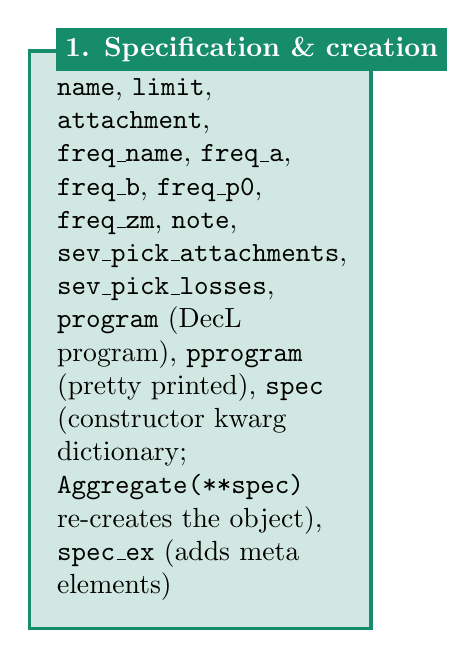
\begin{tikzpicture}
\node [mybox] (box){%
    \begin{minipage}{0.3\textwidth}\raggedright
% {\it italics stuff} \\

\texttt{name},
\texttt{limit},
\texttt{attachment},
\texttt{freq\_name},
\texttt{freq\_a},
\texttt{freq\_b},
\texttt{freq\_p0},
\texttt{freq\_zm},
\texttt{note},
\texttt{sev\_pick\_attachments},
\texttt{sev\_pick\_losses},
\texttt{program} (DecL program),
\texttt{pprogram} (pretty printed),
\texttt{spec} (constructor kwarg dictionary; \texttt{Aggregate(**spec)} re-creates the object),
\texttt{spec\_ex} (adds meta elements)

%    \begin{center}\small{\begin{tabular}{llll}
%        \textit{bs} & right & three & four \\ \hline
%        \textit{log2} & right  & three & four  \\ \hline
%        \textit{sev\_calc} & right  & three & four \\ \hline
%        \textit{left} & right  & three & four \\ \hline
%    \end{tabular}}\end{center}

    \end{minipage}
};
\node[fancytitle] at (box.north west) {1. Specification \& creation};
\end{tikzpicture}


%------------2. UPDATE ---------------
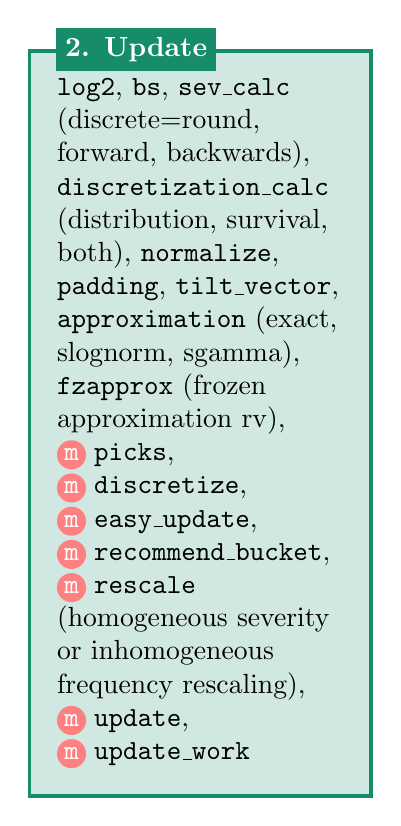
\begin{tikzpicture}
\node [mybox] (box){%
    \begin{minipage}{0.3\textwidth}\raggedright
    
\texttt{log2},
\texttt{bs},
\texttt{sev\_calc} (discrete=round, forward, backwards),
\texttt{discretization\_calc} (distribution, survival, both),
\texttt{normalize},
\texttt{padding},
\texttt{tilt\_vector},
\texttt{approximation} (exact, slognorm, sgamma),
\texttt{fzapprox} (frozen approximation rv),
\texttt{\m picks},
\texttt{\m discretize},
\texttt{\m easy\_update},
\texttt{\m recommend\_bucket},
\texttt{\m rescale} (homogeneous severity or inhomogeneous frequency rescaling),
\texttt{\m update},
\texttt{\m update\_work}

    \end{minipage}
};
\node[fancytitle] at (box.north west) {2. Update};
\end{tikzpicture}


%------------ 3. MOMENTS ---------------
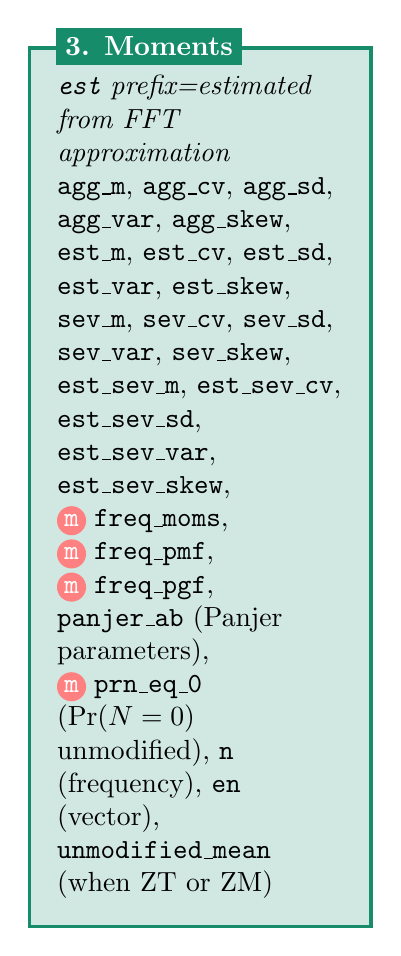
\begin{tikzpicture}
\node [mybox] (box){%
    \begin{minipage}{0.3\textwidth}\raggedright

{\it \texttt{est} prefix=estimated from FFT approximation} \\
\texttt{agg\_m},
\texttt{agg\_cv},
\texttt{agg\_sd},
\texttt{agg\_var},
\texttt{agg\_skew}, \\
\texttt{est\_m},
\texttt{est\_cv},
\texttt{est\_sd},
\texttt{est\_var},
\texttt{est\_skew}, \\
\texttt{sev\_m},
\texttt{sev\_cv},
\texttt{sev\_sd},
\texttt{sev\_var},
\texttt{sev\_skew}, 
\texttt{est\_sev\_m},
\texttt{est\_sev\_cv},
\texttt{est\_sev\_sd},
\texttt{est\_sev\_var},
\texttt{est\_sev\_skew},  
\texttt{\m freq\_moms},
\texttt{\m freq\_pmf},
\texttt{\m freq\_pgf},
\texttt{panjer\_ab} (Panjer parameters),
\texttt{\m prn\_eq\_0} ($\Pr(N=0)$ unmodified),
\texttt{n} (frequency),
\texttt{en} (vector),
\texttt{unmodified\_mean} (when ZT or ZM)

    \end{minipage}
};
\node[fancytitle] at (box.north west) {3. Moments};
\end{tikzpicture}


%------------ 4. STATISTICAL FUNCTIONS ---------------
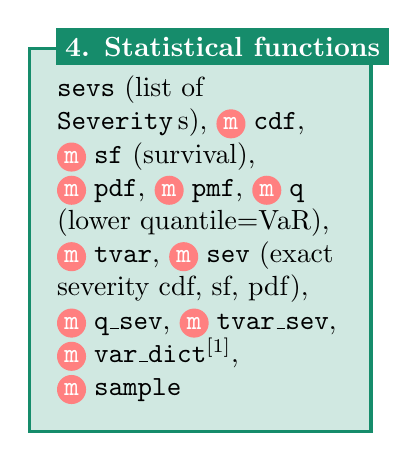
\begin{tikzpicture}
\node [mybox] (box){%
    \begin{minipage}{0.3\textwidth}\raggedright

\texttt{sevs} (list of \texttt{Severity}\,s),
\texttt{\m cdf},
\texttt{\m sf} (survival),
\texttt{\m pdf},
\texttt{\m pmf},
\texttt{\m q} (lower quantile=VaR),
\texttt{\m tvar},
\texttt{\m sev} (exact severity cdf, sf, pdf),
\texttt{\m q\_sev},
\texttt{\m tvar\_sev},
\texttt{\m var\_dict}${}^{[1]}$, 
\texttt{\m sample}

    \end{minipage}
};
\node[fancytitle] at (box.north west) {4. Statistical functions};
\end{tikzpicture}


\columnbreak


%------------ 5. VALIDATION ---------------
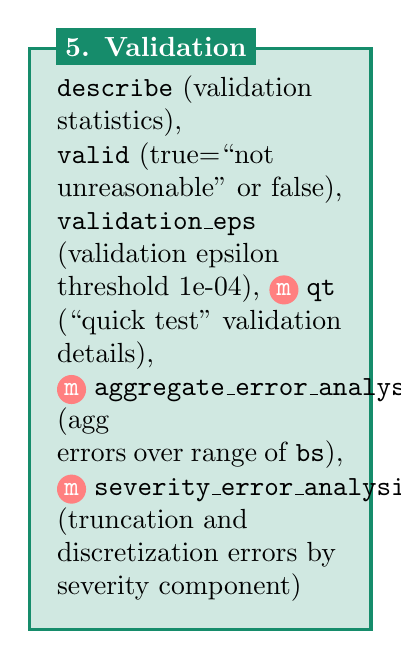
\begin{tikzpicture}
\node [mybox] (box){%
    \begin{minipage}{0.3\textwidth}\raggedright

\texttt{describe} (validation statistics),    \\
\texttt{valid} (true=``not unreasonable'' or false), \\
\texttt{validation\_eps} (validation epsilon threshold 1e-04),
\texttt{\m qt} (``quick test'' validation details),
\texttt{\m aggregate\_error\_analysis} (agg errors over range of \texttt{bs}),
\texttt{\m severity\_error\_analysis} (truncation and discretization errors by severity component)
    
    \end{minipage}
};
\node[fancytitle] at (box.north west) {5. Validation};
\end{tikzpicture}


%------------ 6. OUTPUT ---------------
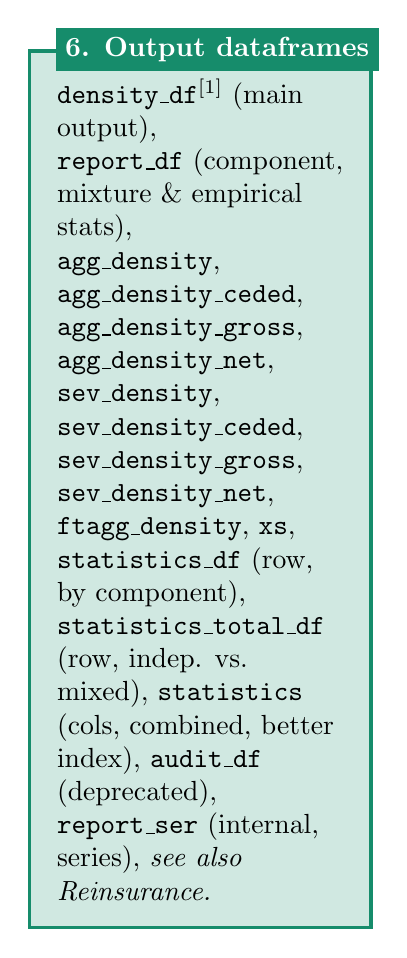
\begin{tikzpicture}
\node [mybox] (box){%
    \begin{minipage}{0.3\textwidth}\raggedright

\texttt{density\_df}${}^{[1]}$ (main output), \\
\texttt{report\_df} (component, mixture \& empirical stats), \\
\texttt{agg\_density},
\texttt{agg\_density\_ceded},
\texttt{agg\_density\_gross},
\texttt{agg\_density\_net},
\texttt{sev\_density},
\texttt{sev\_density\_ceded},
\texttt{sev\_density\_gross},
\texttt{sev\_density\_net},
\texttt{ftagg\_density},
\texttt{xs},
\texttt{statistics\_df} (row, by component),
\texttt{statistics\_total\_df} (row, indep. vs. mixed),
\texttt{statistics} (cols, combined, better index),
\texttt{audit\_df} (deprecated),
\texttt{report\_ser} (internal, series),  {\it see also Reinsurance.}

    \end{minipage}
};
\node[fancytitle] at (box.north west) {6. Output dataframes};
\end{tikzpicture}


%------------ 7. REINSURANCE ---------------
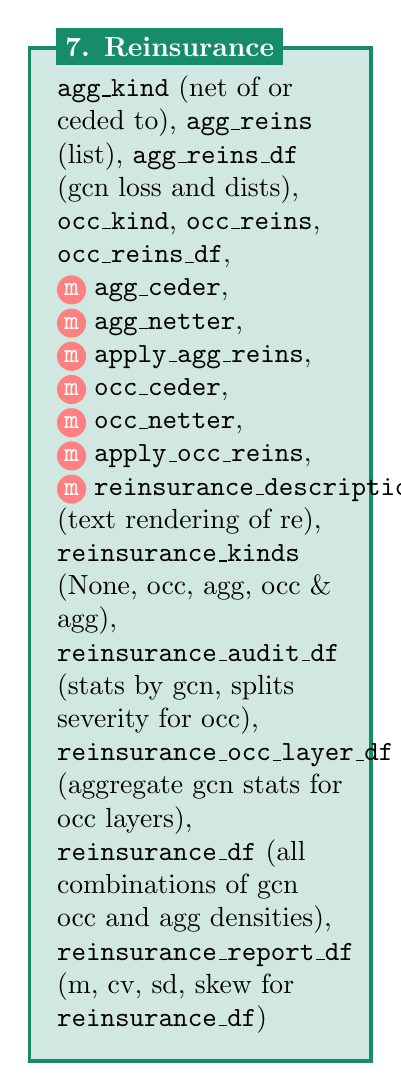
\begin{tikzpicture}
\node [mybox] (box){%
    \begin{minipage}{0.3\textwidth}\raggedright

\texttt{agg\_kind} (net of or ceded to),
\texttt{agg\_reins} (list),
\texttt{agg\_reins\_df} (gcn loss and dists),
\texttt{occ\_kind},
\texttt{occ\_reins},
\texttt{occ\_reins\_df},
\texttt{\m agg\_ceder},
\texttt{\m agg\_netter},
\texttt{\m apply\_agg\_reins},
\texttt{\m occ\_ceder},
\texttt{\m occ\_netter},
\texttt{\m apply\_occ\_reins},
\texttt{\m reinsurance\_description} (text rendering of re),
\texttt{reinsurance\_kinds} (None, occ, agg, occ \& agg),
\texttt{reinsurance\_audit\_df} (stats by gcn, splits severity for occ),
\texttt{reinsurance\_occ\_layer\_df} (aggregate gcn stats for occ layers),
\texttt{reinsurance\_df} (all combinations of gcn occ and agg densities),
\texttt{reinsurance\_report\_df} (m, cv, sd, skew for \texttt{reinsurance\_df}) 

    \end{minipage}
};
\node[fancytitle] at (box.north west) {7. Reinsurance};
\end{tikzpicture}



\columnbreak


%------------ 8. VISUALIZTION ---------------
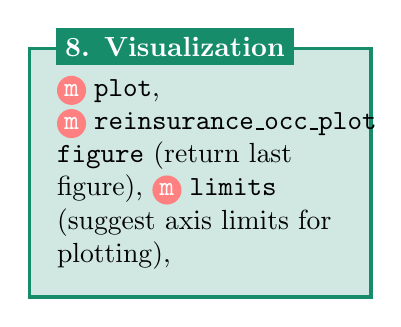
\begin{tikzpicture}
\node [mybox] (box){%
    \begin{minipage}{0.3\textwidth}\raggedright

\texttt{\m plot},
\texttt{\m reinsurance\_occ\_plot}
\texttt{figure} (return last figure),
\texttt{\m limits} (suggest axis limits for plotting),

    \end{minipage}
};
\node[fancytitle] at (box.north west) {8. Visualization};
\end{tikzpicture}


%------------ 9. RISK ---------------
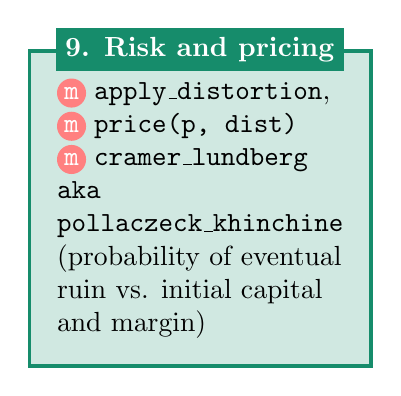
\begin{tikzpicture}
\node [mybox] (box){%
    \begin{minipage}{0.3\textwidth}\raggedright

\texttt{\m apply\_distortion},
\texttt{\m price(p, dist)}
\texttt{\m cramer\_lundberg aka pollaczeck\_khinchine} (probability of eventual ruin vs. initial capital and margin)

    \end{minipage}
};
\node[fancytitle] at (box.north west) {9. Risk and pricing};
\end{tikzpicture}


%------------  10. APPROXIMATIONS ---------------
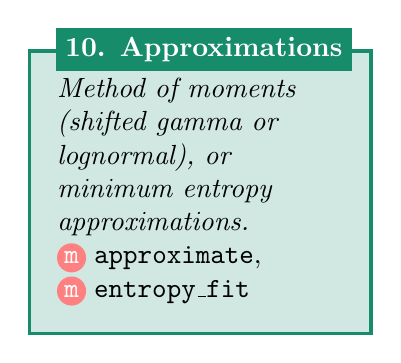
\begin{tikzpicture}
\node [mybox] (box){%
    \begin{minipage}{0.3\textwidth}\raggedright

{\it Method of moments (shifted gamma or lognormal), or minimum entropy approximations.} \\
\texttt{\m approximate},
\texttt{\m entropy\_fit}

    \end{minipage}
};
\node[fancytitle] at (box.north west) {10. Approximations};
\end{tikzpicture}


%------------ 11. META ---------------
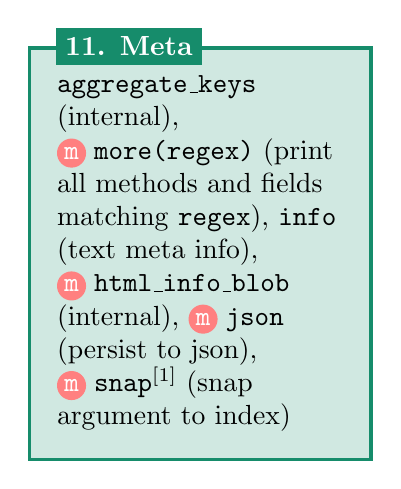
\begin{tikzpicture}
\node [mybox] (box){%
    \begin{minipage}{0.3\textwidth}\raggedright

\texttt{aggregate\_keys} (internal),
\texttt{\m more(regex)} (print all methods and fields matching \texttt{regex}),
\texttt{info} (text meta info),
\texttt{\m html\_info\_blob} (internal),
\texttt{\m json} (persist to json),
\texttt{\m snap}${}^{[1]}$ (snap argument to index)
    
    \end{minipage}
};
\node[fancytitle] at (box.north west) {11. Meta};
\end{tikzpicture}

\bigskip \raggedright
{\bf Notes:} 

[0]: Arguments \texttt{sev\_pick\_attachments=None, sev\_pick\_losses=None, } omitted; see help. 

[1]: matches \texttt{Portfolio} 

Any vectorizable input accepts numeric or iterable datatypes.  

Abbreviations: gcn=gross (subject), ceded, and net; stats: m=mean, cv=coefficient of variation, sd=standard deviation, var=variance, skew(ness); VaR=value-at-risk


% \vskip .25truein
% FOOTER
\makefooter



\end{multicols*}

\end{document}
